\subsection{What changes the outcome: information or learning design?}
\label{sec:design}

The two channels make opposite predictions about interventions. If low trading
were sustained by punishment, degrading the information traders use to
monitor each other should restore competition, and the content of their memory
should matter. If it is pruning, information is irrelevant and changes to the
learning procedure should matter. Table~\ref{tab:design} and
Figure~\ref{fig:design} report treatments in the standard Kyle market, each
against the residual-memory baseline ($\Delta=\ResidDeltaInt$).

\paragraph{Information does not matter.} Blurring the order flow that traders
observe with noise of twice the noise-trading volume leaves the outcome
unchanged ($\Delta=\OpaqueDeltaInt$). Replacing the informative memory with a
\emph{random} state that carries no information at all, but has the same
number of states, reproduces it ($\Delta=\RandomMemDeltaInt$). The difference
between forward-looking learners with and without memory
(\ResidDeltaInt{} versus \NoneDeltaInt{}) is therefore a matter of table size:
more states mean fewer updates per entry and more room for the selection effect
of Section~\ref{sec:mechanism}, not more information to coordinate on.

\paragraph{Learning design matters.} The step size alone sets the level of the
outcome (Figure~\ref{fig:alpha}): with residual memory the index is
$\AlphaResidLow$, $\AlphaResidMid$ and $\AlphaResidHigh$ at $\alpha=0.05$,
$0.15$ and $0.3$, and without memory $\AlphaNoneLow$, $\AlphaNoneMid$ and
$\AlphaNoneHigh$, running from competition to beyond the cartel, with no
punishment at any step size, as the square-root law of
Section~\ref{sec:mechanism} predicts. Two further changes to the learning
rule move the outcome substantially. Counterfactual updating, which removes the selection
effect, eliminates the supracompetitive outcome: forward-looking learners end
at $\Delta=\CfResidDeltaInt$ with residual memory and $\CfNoneDeltaInt$ without,
that is, at (marginally beyond) the competitive level, with price
informativeness at its Nash value ($\Delta$ informativeness
$\CfResidDeltaInfo$). The market, the agents' information and the exploration
schedule are unchanged; only the update rule differs. Per-entry decaying step sizes
change even the sign: learners \emph{over}-trade relative to Nash
($\Delta=\VisitsResidual$ with residual memory, $\VisitsNone$ without),
because step sizes shrink while heavy exploration still depresses the market
maker's price impact.

\paragraph{When collusion means trading more.} Adding two passive informed
traders who play the Nash strategy reverses the benchmarks: facing outside
competition, the two learners would maximise their joint profit by trading
\emph{more} than their Nash intensity (aggregate $\PassiveAggColl$ versus
$\PassiveAggNash$), because extra informed flow lowers the market maker's price
impact. A collusive force should push them up. Instead they trade
$\PassiveAgg$, half their Nash intensity, moving away from the cartel and
earning $\PassiveProfitPct$\% less than in the Nash equilibrium. The learners
under-trade whichever side of Nash the collusive outcome lies on, which is what a
learning bias predicts and the opposite of what collusion predicts. (In the
collusion index this appears as $\Delta=\PassiveDeltaInt$, which is why
Table~\ref{tab:design} should be read with the benchmarks in mind.)

\ECfloat{sections/fig_alpha}

\begin{figure}[t]
  \centering
  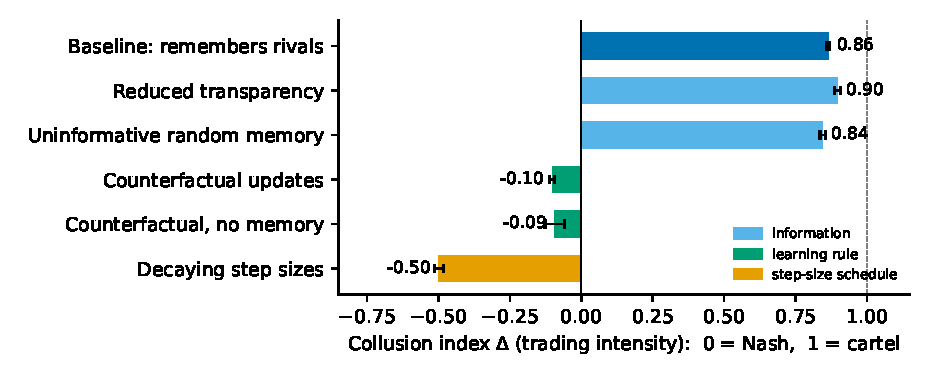
\includegraphics[width=0.85\linewidth]{figures/fig_design.pdf}
  \caption{Interventions in the standard Kyle market. Treatments that change
  what traders observe leave the outcome unchanged; treatments that change how
  they learn move it to, or past, competition.}
  \label{fig:design}
\end{figure}

\begin{table}[t]
  \centering
  \small
  \resizebox{\linewidth}{!}{\begin{tabular}{lcccc}
\toprule
Treatment ($\xi=0$, $I=2$) & $\Delta$ intensity & $\Delta$ profit & Rival $\Delta\beta_1$ & Deviator gain \\
\midrule
Random memory, 35 states & $0.84 \pm 0.01$ & $0.45 \pm 0.03$ & $0.000 \pm 0.000$ & $0.052 \pm 0.004$ \\
Random memory, myopic & $1.16 \pm 0.01$ & $0.11 \pm 0.02$ & $0.000 \pm 0.000$ & $0.107 \pm 0.006$ \\
Counterfactual updates, residual memory & $-0.10 \pm 0.01$ & $-0.44 \pm 0.03$ & $-0.001 \pm 0.002$ & $0.020 \pm 0.003$ \\
Counterfactual updates, no memory & $-0.09 \pm 0.03$ & $-0.34 \pm 0.08$ & $0.000 \pm 0.000$ & $0.015 \pm 0.002$ \\
Counterfactual updates, residual, myopic & $-0.10 \pm 0.01$ & $-0.44 \pm 0.03$ & $-0.001 \pm 0.002$ & $0.019 \pm 0.003$ \\
Reduced transparency (disclosure noise $2\sigma_u$) & $0.90 \pm 0.01$ & $0.46 \pm 0.03$ & $-0.002 \pm 0.003$ & $0.058 \pm 0.004$ \\
Two passive Nash traders & $-1.26 \pm 0.01$ & $-8.56 \pm 0.09$ & $0.001 \pm 0.003$ & $0.036 \pm 0.003$ \\
DQN & $-0.36 \pm 0.07$ & $-0.89 \pm 0.13$ & $-0.000 \pm 0.004$ & $0.026 \pm 0.008$ \\
DQN, myopic & $-0.17 \pm 0.03$ & $-0.46 \pm 0.06$ & $-0.001 \pm 0.005$ & $0.014 \pm 0.007$ \\
PPO & $-0.02 \pm 0.09$ & $-0.27 \pm 0.12$ & $0.000 \pm 0.000$ & $0.028 \pm 0.008$ \\
PPO, myopic & $-0.28 \pm 0.05$ & $-0.51 \pm 0.10$ & $0.000 \pm 0.000$ & $0.012 \pm 0.006$ \\
\bottomrule
\end{tabular}}
  \caption{Treatments in the standard Kyle market ($\xi=0$, $I=2$, residual
  memory unless noted, $6\times10^6$ periods, 200 markets). Baseline:
  $\Delta$ intensity $\ResidDeltaInt$. 95\% CIs.}
  \label{tab:design}
\end{table}
